\documentclass[12pt,a4paper]{article}
\usepackage[utf8]{inputenc}
\usepackage[russian]{babel}
\usepackage[OT1]{fontenc}
\usepackage{mathtools}
\usepackage{amsfonts}
\usepackage{amssymb}
\usepackage{enumitem}
\usepackage{alltt}
\usepackage{graphicx}
\usepackage{indentfirst}
\usepackage{caption}
\usepackage{float}
\usepackage{wrapfig}
\usepackage{physics}
\usepackage{multirow}
\usepackage{longtable}
\usepackage{amsmath,amsfonts,amssymb,amsthm,mathtools}
\usepackage{icomma}
\setlength{\parindent}{0.75cm}
\graphicspath{{pictures/}}
\DeclareGraphicsExtensions{.png, .jpg}
\usepackage[left=15mm,right=15mm,top=2cm,bottom=2cm]{geometry}
\author{Глотов Алексей}
\begin{document}
\newpage
\begin{center}
\footnotesize{{ГОСУДАРСТВЕННОЕ АВТОНОМНОЕ ОБРАЗОВАТЕЛЬНОЕ УЧРЕЖДЕНИЕ}\break
{ВЫСШЕГО ОБРАЗОВАНИЯ}
\break
{\bf {МОСКОВСКИЙ ФИЗИКО-ТЕХНИЧЕСКИЙ ИНСТИТУТ}}
\break
\small{(НАЦИОНАЛЬНЫЙ ИССЛЕДОВАТЕЛЬСКИЙ УНИВЕРСИТЕТ)}}
\break
\hfill \break
\hfill \break
\begin{center}
\normalsize{Кафедра общей физики}
\end{center}
\hfill \break
\hfill \break
\hfill \break
\hfill \break

\begin{center}
\normalsize {Лабораторная работа 5.5.5}
\end{center}
\hfill \break\\
\large{\textbf{Компьютерная сцинтилляционная $\gamma$ -спектрометрия}}
\end{center}
\begin{flushleft}
\hfill \break
\hfill \break
\hfill \break
\hfill \break
\hfill \break
\hfill \break
\hfill \break
\hfill \break
\hfill \break
\hfill \break
\hangindent=10cm
\normalsize{Преподаватель:} \;\;\;\;
\normalsize{к.ф.-м.н. Юрьев Ю.В.}\\
\hfill \break
\normalsize{Обучающийся:} \;\;\;\;\;
\normalsize{Глотов А.А} \\
\hfill \break
\end{flushleft}
\hfill \break
\hfill \break
\hfill \break
\hfill \break
\hfill \break
\hfill \break
\hfill \break
\hfill \break
\hfill \break
\hfill \break
\hfill \break

\begin{center}
Долгопрудный \break
 2023
\end{center}

\thispagestyle{empty}


\newpage
\section{Введение}

\subsection{Аннотация}

В квантовой физике, в отличие от классической, энергия частицы обладает дискретными значениями (не непрерывным набором значений). Это выражается в испускании электронами квантов света только определённых энергий. Это происходит при смене электроном энергетического уровня. Ввиду этого, при рассмотрении спектра энергии, испускаемых гамма квантов можно увидеть ряд пиков. Такой эксперимент называется гамма-спектрометрией.

     \textbf{Цель:} при помощи компьютерной сцинтилляционной гамма-спектрометрии исследовать энергетические спектры различных веществ.


\subsection{Теоретические сведения}

\textbf{Фотоэффект} - это процесс взаимодействия гамма-кванта с электроном, связанным с атомом, при котором электрону передается вся энергия гамма-кванта. При этом электрону сообщается кинетическая энергия $T_e=E_\gamma-I_i$, где $E_\gamma$ -- энергия гамма-кванта, $I_i$ -- потенциал ионизации $i$-той оболочки атома. Фотоэффект особенно существенен для тяжелых веществ, где он идет с заметной вероятностью даже при высоких энергиях гамма-квантов. В легких веществах фотоэффект становится заметен лишь при относительно небольших энергиях гамма-квантов.  \par
\textbf{Эффект Комптона} - это упругое рассеяние фотона на свободном электроне, сопровождающееся изменением длины волны фотона. Максимальная энергия образующихся комптоновских электронов соответствует рассеянию гамма-квантов на $180^\circ$ и равна
\begin{equation}
E_{\max}=\frac{\eta\omega}{1+\frac{mc^2}{2\eta\omega}}.
\end{equation}
\textbf{Процесс образования электрон-позитронных пар.}
При достаточно высокой энергии гамма-кванта наряду с фотоэффектом и эффектом Комптона может происходить третий вид взаимодействия гамма-квантов с веществом -- образование электрон-позитронных пар. Процесс образования пар не может происходить в пустоте, так как в этом случае не выполняются законы сохранения энергии и импульса. В присутствии ядра или электрона процесс образования пары гамма-квантов возможен, так как можно распределить энергию и импульс гамма-кванта между тремя частицами без противоречия с законами сохранения. При этом если процесс образования пары идет в кулоновском поле ядра или протона, то энергия образующегося ядра отдачи оказывается весьма малой, так что пороговая энергия гамма-кванта $E_0$, необходимая для образования пары, практически совпадает с удвоенной энергией покоя электрона $E_0\cong 2mc^2=1.022$ МэВ.\par
Появившийся в результате процесса образования пар электрон свою энергию на ионизацию среды. Таким образом, вся энергия электрона остается в детекторе. Позитрон будет двигаться до тех пор, пока практически не остановится, а затем аннигилирует с электроном среды, в результате чего появятся два гамма-кванта. Т.е., кинетическая энергия позитрона также останется в детекторе. Далее возможны три варианта развития событий:
\begin{enumerate}
\item оба родившихся гамма-кванта не вылетают из детектора, и тогда вся энергия первичного гамма-кванта останется в детекторе, а в спектре появится пик с $E=E_{\gamma}$;
\item один из родившихся гамма-квантов покидает детектор, и в спектре появляется пик, соответствующий энергии $E=E_{\gamma}-E_0$, где $E_0=mc^2=511$ кэВ;
\item оба родившихся гамма-кванта покидают детектор, и в спектре появляется пик, соотвествующий энергии $E=E_{\gamma}-2E_0$, где $2E_0=2mc^2=1022$ кэВ.
\end{enumerate}
Таким образом, любой спектр, получаемый с помощью гамма-спектрометра, описывается несколькими компонентами, каждая из которых связана с определенным физическим процессом. Как описано выше, основными физическими процессами взаимодействия гамма-квантов с веществом является фотоэффект, эффект Комптона и образование электрон-позитронных пар, и каждый из них вносит свой вклад в образование спектра. Помимо этих процессов, добавляется \textit{экспонента}, связанная с наличием фона, \textit{пик характеристического излучения}, возникающий при взаимодействии гамма-квантов с окружающим веществом, а также \textit{пик обратного рассеяния}, образующийся при энергии квантов $E_{\gamma}\gg mc^2/2$ в результате рассеяния гамма-квантов на большие углы на материалах  конструктивных элементов детектора и защиты. Положение пика обратного рассеяния определяется по формуле:
\begin{equation}
E_{\text{обр}}=\frac{E}{1+2E/mc^2},
\label{eq:Ereverse}
\end{equation}
где $E$ -- энергия фотопика.\par
\paragraph{Энергетическое разрешение спектрометра.} Даже при поглощении частиц с одинаковой энергией амплитуда импульса на выходе фотоприёмника сцинтилляционного детектора меняется от события к событию. Это связано:
\begin{enumerate}
\item со статистическим характером процессов сбора фотонов на фотоприёмнике и последующего усиления,
\item с различной вероятностью доставки фотона к фотоприемнику из разных точек сцинтиллятора,
\item с разбросом высвечиваемого числа фотонов
\end{enumerate}
\par
В результате в набранном спектре линия (которая для идеального детектора представляла бы дельта-функцию) оказывается размытой, её часто описывают гауссианом.\par
Энергетическим разрешением спектрометра называется величина
\begin{equation}
R_i=\frac{\Delta E_i}{E_i},
\end{equation}
где $\Delta E_i$ -- ширина пика полного поглощения, измеренная на половине высоты, $E_i$ -- энергия регистрируемого $\gamma$-излучения. Значение $E_i$ пропорционально среднему числу фотонов $\overline{n_i}$ на выходе ФЭУ, т.е.:
\begin{equation}
E_i=\alpha\overline{n_i}.
\label{eq:4}
\end{equation}
\par
Полуширина пика полного поглощения $\Delta E_i$ пропорциональна среднеквадратичной флуктуации $\overline{\Delta n_i}$. Т.к. $n_i$ является дискретной случайной величиной, которая распределена по закону Пуассона, то $\overline{\Delta n_i}=\sqrt{\overline{n_i}}$ и поэтому
\begin{equation}
\Delta E_i=\alpha\overline{\Delta n_i}=\alpha\sqrt{\overline{n_i}}.
\label{eq:5}
\end{equation}
\par
Из (\ref{eq:4}), (\ref{eq:5}) получаем, что
\begin{equation}
R_i=\frac{\Delta E_i}{E_i}=\frac{\text{const}}{\sqrt{E_i}}.
\label{eq:6}
\end{equation}
\par
Поскольку энергетическое разрешение зависит от энергии, его следует указывать для конкретной энергии. Чаще всего разрешение указывают для энергии гамма-линии $^{137}\text{Cs}$ (661.7 кэВ).

\newpage
\section{Результаты измерений и обработка данных}

Измерим спектры излучения 5 различных материалов, а также спектр фонового излучения. Нанесем точки на график


\begin{figure}[H]
\begin{minipage}[h]{0.45\linewidth}
\center{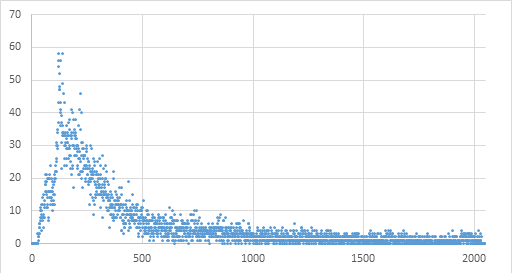
\includegraphics[width=1\linewidth]{5.5.5-1}} Рис.1 Спектр фонового излучения \\
\end{minipage}
\hfill
\begin{minipage}[h]{0.45\linewidth}
\center{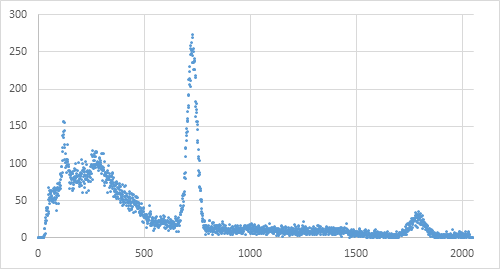
\includegraphics[width=1\linewidth]{5.5.5-2}} \\ Рис.2 Спектр излучения Na-22
\end{minipage}
\end{figure}

\begin{figure}[H]
\begin{minipage}[h]{0.45\linewidth}
\center{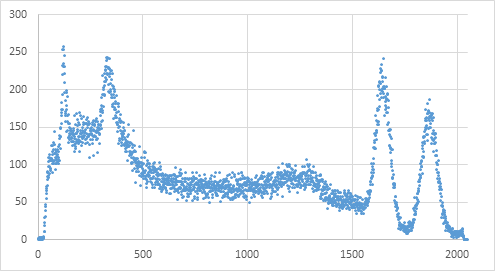
\includegraphics[width=1\linewidth]{5.5.5-3}} Рис.3 Спектр излучения Co-60\\
\end{minipage}
\hfill
\begin{minipage}[h]{0.45\linewidth}
\center{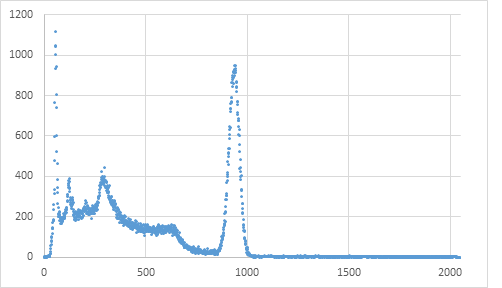
\includegraphics[width=1\linewidth]{5.5.5-4}} \\ Рис.4 Спектр излучения Cs-137
\end{minipage}
\end{figure}

\begin{figure}[H]
\begin{minipage}[h]{0.45\linewidth}
\center{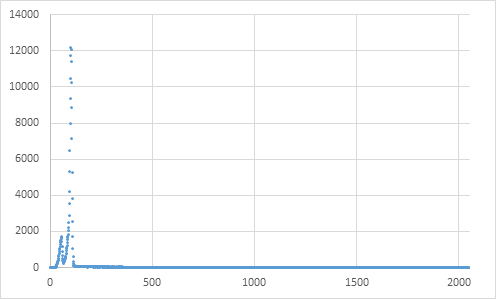
\includegraphics[width=1\linewidth]{5.5.5-5}} Рис.5 Спектр излучения Am-241 \\
\end{minipage}
\hfill
\begin{minipage}[h]{0.45\linewidth}
\center{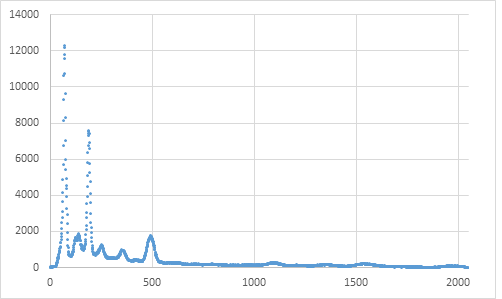
\includegraphics[width=1\linewidth]{5.5.5-6}} \\ Рис.6 Спектр излучения Eu-152
\end{minipage}
\end{figure}

Используя спектры Na-22, Co060 и Cs-137 как калибровочные, построим график энергии излучения E от номера канала счетной программы N (рис.7).

\begin{center}
\begin{tabular}{|c|c|c|c|c|c|}
\hline 
Вещество & Na-22 & Na-22 & Co-60 & Co-60 & Cs-137 \\ 
\hline 
№ канала & 725 & 1793 & 1641 & 1869 & 935 \\ 
\hline 
E, кэВ & 511.0 & 1274.0 & 1173.2 & 1332.5 & 661.7 \\ 
\hline 
\end{tabular} 
\end{center}

\begin{figure}[H]
\begin{minipage}[h]{0.49\linewidth}
\center{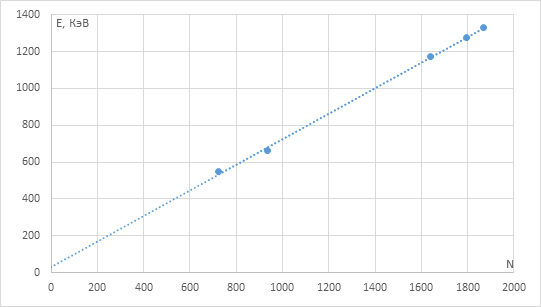
\includegraphics[width=1\linewidth]{5.5.5-7}} Рис.7 Калибровочный график \\
\end{minipage}
\hfill
\begin{minipage}[h]{0.49\linewidth}
\center{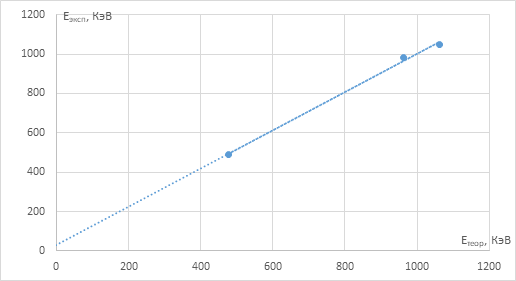
\includegraphics[width=1\linewidth]{5.5.5-8}} \\ Рис.8 Максимальная энергия Комптоновского рассеяния
\end{minipage}
\end{figure}

С помощью расчетных программ вычислим значения коэффициентов прямой и оценим погрешности	

	
\begin{large}
E = k $\cdot$ N + b

\begin{center}
$k = (0.718 \pm 0.003) $ кэВ \;\;\;\;\;\;\;\; $b = (9 \pm 5)$ кэВ
\end{center}
\end{large}

Теперь, зная координаты вершины пиков излучения и их ширину в номерах канала, а также калибровочную зависимость, пересчитаем все известные нам пики всех материалов в энергию

\begin{center}
\begin{tabular}{|c|c|c|c|c|c|}
\hline 
Вещество & N & $\Delta$N & E, кЭв & $\Delta$E, кэВ & R \\ 
\hline 
Na-22 & 725 & 53 & 512 $\pm$ 7 & 29 $\pm$ 5 & 0.057 $\pm$ 0.009 \\ 
\hline 
Na-22 & 1793 & 48 & 1280 $\pm$ 10 & 25 $\pm$ 4 & 0.020 $\pm$ 0.004 \\ 
\hline 
Co-60 & 1641 & 48 & 1170 $\pm$ 10 & 54 $\pm$ 9 & 0.046 $\pm$ 0.004 \\ 
\hline 
Co-60 & 1869 & 76 & 1330 $\pm$ 12 & 46 $\pm$ 7 & 0.034 $\pm$ 0.004 \\ 
\hline 
Cs-137 & 935 & 60 & 648 $\pm$ 7 & 34 $\pm$ 5 & 0.053 $\pm$ 0.007 \\ 
\hline 
Am-241 & 100 & 11 & 63 $\pm$ 3 & 8 $\pm$ 2 & 0.13 $\pm$ 0.08 \\ 
\hline 
Eu-152 & 67 & 8 & 39  $\pm$ 3 & 6 $\pm$ 1 & 0.15 $\pm$ 0.13 \\ 
\hline 
Eu-152 & 188 & 15 & 126 $\pm$ 16 & 11 $\pm$ 3 & 0.09 $\pm$ 0.04 \\ 
\hline 
\end{tabular} 
\end{center}

Далее определим энергию края комптоновского рассеяния. Построим график зависимости экспериментальных значений от теоретических (рис.8)

\begin{center}
\begin{tabular}{|c|c|c|c|}
\hline 
Вещество & Na-22 & Co-60 & Cs-137 \\ 
\hline 
$E_\text{теор}$, кЭв & 1062 & 963 & 477 \\ 
\hline 
$E_\text{эксп}$, кЭв & 1050 $\pm$ 50 & 980 $\pm$ 50 & 490 $\pm$ 30 \\ 
\hline 
\end{tabular} 
\end{center}

Построим график $R = f(\frac{1}{E})$

\begin{figure}[H]
	\begin{center}
	\vspace{-1.9ex}
		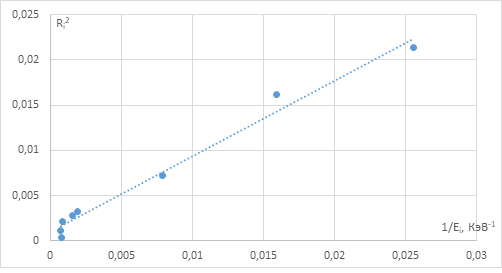
\includegraphics{5.5.5-9}
		\caption{Рис.9 Зависимость квадрата разрешения от обратной энергии}
	\end{center}
\end{figure}

\section{Обсуждение результатов и выводы}
	
     В ходе работы, при помощи компьютерной сцинтилляционной гамма-спектрометрии мы определили энергетические спектры для различных веществ: Na-22, Co-60, Cs-137, Eu-152, Am-241. Мы определили для этих веществ: энергии пиков полного поглощения, энергии краёв комптоновского рассеяния, энергии обратного излучения. А также определили величину характеристического излучения.

\end{document}